\documentclass[a4paper, 12pt]{article}
\usepackage{amsmath, amsthm, amssymb, bm}
\usepackage{graphicx}
\usepackage{makeidx}
\usepackage{float}
\usepackage[top=1.5in, bottom=1.5in, left=1in, right=1in]{geometry}
\makeidx
\setlength\parindent{0pt} % Removes all indentation from paragraphs

\renewcommand{\labelenumi}{\alph{enumi}.} % Make numbering in the enumerate environment by letter rather than number (e.g. section 6)
\begin{document}
%%%%%%%%%%%%%%%%%%%%%%%%%%%%%%%%%%%%%%%%%
% University Assignment Title Page 
% LaTeX Template
% Version 1.0 (27/12/12)
%
% This template has been downloaded from:
% http://www.LaTeXTemplates.com
%
% Original author:
% WikiBooks (http://en.wikibooks.org/wiki/LaTeX/Title_Creation)
%
% License:
% CC BY-NC-SA 3.0 (http://creativecommons.org/licenses/by-nc-sa/3.0/)
% 
% Instructions for using this template:
% This title page is capable of being compiled as is. This is not useful for 
% including it in another document. To do this, you have two options: 
%
% 1) Copy/paste everything between \begin{document} and \end{document} 
% starting at \begin{titlepage} and paste this into another LaTeX file where you 
% want your title page.
% OR
% 2) Remove everything outside the \begin{titlepage} and \end{titlepage} and 
% move this file to the same directory as the LaTeX file you wish to add it to. 
% Then add \input{./title_page_1.tex} to your LaTeX file where you want your
% title page.
%
%%%%%%%%%%%%%%%%%%%%%%%%%%%%%%%%%%%%%%%%%

%----------------------------------------------------------------------------------------
% PACKAGES AND OTHER DOCUMENT CONFIGURATIONS
%----------------------------------------------------------------------------------------
\begin{titlepage}

\newcommand{\HRule}{\rule{\linewidth}{0.5mm}} % Defines a new command for the horizontal lines, change thickness here
\vspace*{40mm}
\center % Center everything on the page
 
 %----------------------------------------------------------------------------------------
 %  HEADING SECTIONS
 %----------------------------------------------------------------------------------------

 \textsc{\LARGE Portland State University}\\[1.5cm] % Name of your university/college
 \textsc{\Large CS350 }\\[0.5cm] % Major heading such as course name
 \textsc{\large Algorithms And Complexity}\\[0.5cm] % Minor heading such as course title

 %----------------------------------------------------------------------------------------
 %  TITLE SECTION
 %----------------------------------------------------------------------------------------

 \HRule \\[0.4cm]
 { \huge \bfseries ConvexHull Analysis:\\ BruteForce vs. QuickHull}\\[0.4cm] % Title of your document
 \HRule \\[1.5cm]
  
  %----------------------------------------------------------------------------------------
  % AUTHOR SECTION
  %----------------------------------------------------------------------------------------

  \begin{minipage}{0.4\textwidth}
  \begin{flushleft} \large
  \emph{Author:}\\
  Wes \textsc{Risenmay}\\ % Your name
  Josh \textsc{Willhite} % Your name
  \end{flushleft}
  \end{minipage}
  ~
  \begin{minipage}{0.4\textwidth}
  \begin{flushright} \large
  \emph{Instructor:} \\
  Dr. Andrew \textsc{Black} % Supervisor's Name
  \end{flushright}
  \end{minipage}\\[4cm]

  % If you don't want a supervisor, uncomment the two lines below and remove the section above
  %\Large \emph{Author:}\\
  %John \textsc{Smith}\\[3cm] % Your name

  %----------------------------------------------------------------------------------------
  % DATE SECTION
  %----------------------------------------------------------------------------------------

  {\large \today}\\[3cm] % Date, change the \today to a set date if you want to be precise

  %----------------------------------------------------------------------------------------
  % LOGO SECTION
  %----------------------------------------------------------------------------------------

  %\includegraphics{Logo}\\[1cm] % Include a department/university logo - this will require the graphicx package
   
   %----------------------------------------------------------------------------------------

   \vfill % Fill the rest of the page with whitespace

   \end{titlepage}

\tableofcontents{}
\vspace{10cm}
{
  \section{Objective}
The purpose of this paper is to compare convex hull algorithms specifically, brute force vs. QuickHull.  Our comparison will consist of an analytic time efficiency analysis of the two algorithms followed by actual timing of the algorithms for the same input data. We'll conclude with an explaination of how our predicitions compared to the data.   
  \section{ConvexHull Overview}
  Given a set of points in the XY plane, imagine stretching a rubber band around the set. All of the points that the rubber band touchs are on the convex hull \textit{[Levitin pg.110]}.  
  \begin{figure}[H]
    \begin{center}
    \includegraphics[width=4cm,height=4cm]{rubber_band.png}
  \end{center}
    \caption{Convex hull Example}
    \label{fig:rubber_band}
  \end{figure} 
  Finding the convex hull of a given set ends up being critical in a bunch of different areas, from computer vision to Geographic Information Systems to CAD applications \textit{[Levitin pg.110]}
  \section{Algorithm Explaination}
  \subsection{Brute Force}
The brute force approach to finding the convex hull of a set of points is to use 3 nested loops.  The two outer loops get a point(a) and point(b) which form a line.  The inner loop than calculates the determinant of of the two points which make up the line with a third point(c).  If two of the "c" points are ever on opposite sides of the line (determinant has different sign) than we know line(a-b) can't be on the hull and we move on.   
  \begin{figure}[H]
  \begin{center}
    \includegraphics[width=4cm,height=4cm]{BF_1.png}
\end{center}
\caption{Brute Force Example}
    \label{fig:bf_1}
  \end{figure} 
In the above diagram our the line we're testing would be from A-B. First AxBx1 would be calculated, then AxBx2 would be compared to the first determinant they're the same so the algorithm would continue until AxBx4 is reached. Since the sign of this last determinant does not match the other the line A-B is not on the hull and we can move on to the text the next line.
  \subsection{QuickHull}
  The QuickHull approach is both more elegant and more performant. (1) Find furthest left and right points A,B in the figure below. These two points are guaranteed to be on the hull.  (2) Split the remaining points into two subsets above/below the base edge. (3a) The recursive step starts by finding the furthest point from the base edge, in the below figure it's labeled "Pivot" for the top subset. (3b) Now divide the current set of points into two subsets consisting of points to the right of the line from Pivot->B and points to the left of the line from Pivot->A. (3c) Now call the recursive function twice again, once for the base edge Pivot->B with the associated subset and ponce for the base edge Pivot->A for the associated subset. If there are not points in a subset then stop the recursion. 
  \begin{figure}[H]
  \begin{center}
    \includegraphics[width=5cm,height=5cm]{qh_1.png}
\end{center}
\caption{QuickHull Example}
    \label{fig:qh_1}
  \end{figure} 
  \section{Algorithm Implementation}
  \subsection{Brute Force}

  Our implementation for the brute force algorithm is shown in figure ~\ref{fig:bruteforce} below. There weren't any real issues getting it to work and it's fairly self explainitory.
  \begin{figure}[H]
  \begin{center}
    \includegraphics[width=16cm,height=16cm]{bruteforce.png}
\end{center}
    \caption{Brute Force Convex Hull}
    \label{fig:bruteforce}
  \end{figure} 
  \subsection{QuickHull}
 The implementation of QuickHull on the other hand ended up being very time consuming, mainly due to the difficulties inherint in debugging recusive code.  
  \begin{figure}[H]
  \begin{center}
    \includegraphics[width=9cm,height=6cm]{min_max.png}
  \end{center}
    \caption{Max Min Function}
    \label{fig:min_max}
  \end{figure} 
  The maxmin() function above is used to find the initial base edge composed of the furthest left and right points. Basically just a loop through all points keeping track of the current highest and lowest points. 

  \begin{figure}[H]
  \begin{center}
    \includegraphics[width=18cm,height=1.4cm]{get_det.png}
  \end{center}
    \caption{Calculate Determinant}
    \label{fig:get_det}
  \end{figure} 

  Similar to the brute force case a determinant is used to figure out which side of the line a point is on.  The method above is called each time a new pivot point is found in order to find points that lay either to the left or the right of the resulting triangle.
  
  \begin{figure}[H]
  \begin{center}
    \includegraphics[width=13cm,height=5cm]{get_pivot_point.png}
  \end{center}
    \caption{Get The Pivot Point}
    \label{fig:get_pivot}
  \end{figure}
  Given a subset of points we need to find the pivot (furthest point from the base edge). This ends up being pretty straight forward since we already have a method to calculate the determinant, this can be repurposed in order to get the distance along a normal vector from the base edge to each point in the current set.  


  \begin{figure}[H]
  \begin{center}
    \includegraphics[width=14cm,height=8cm]{get_subset.png}
  \end{center}
    \caption{Get The Resulting Subset}
    \label{fig:get_subset}
  \end{figure}
One of the keys to getting QuickHull to work was figuring out which of the points in a given subset should be used to create the next subsets for the recursive call.  This is again accomplished by looping through the remaining points and calling the determinanat method on each point, points to the right of a line on the upper right side of the pivot will have a positive determinant, points on the upper left side a negative determinant.  For the lower hull these values are swithced.

  \begin{figure}[H]
  \begin{center}
    \includegraphics[width=14cm,height=16cm]{dome.png}
  \end{center}
    \caption{Recursive Dome Function}
    \label{fig:dome}
  \end{figure}

The heart of this implementation of QuickHull is the recursive dome method. It taked the current edge, set of points and a flag indicating if the current subset is int he upper or lower hull. Next we find the pivot point and figure out if the resulting edges are on the left or the right side of the calling edge. and finally if there are any points in the new resulting subsets we can either call the dome function again or stop the recursion. 

  \begin{figure}[H]
  \begin{center}
    \includegraphics[width=14cm,height=4.7cm]{quickhull.png}
  \end{center}
    \caption{Setup And Call Dome}
    \label{fig:quickhull}
  \end{figure}

  The final component of this QuickHull implementation is the above initialization function appropriately called quickhull.  As mentioned earlier we need to first find the furthest left and right points then proceed to divide the whole set into upper and lower subsets and finally make the calls to the recursive dome function with the appropriate point sets and flag. 

  \section{Analysis of Time Complexity}
  \subsection{Brute Force}
  Our brute force implementation is composed of 3 loops, each of which iterates through every point in the input. The basic operation for our algorithm is calculating the determinant which occurs in the inner most loop.
  \begin{center}
    \begin{align*}
      C(n) &= \sum\limits_{i=1}^n \sum\limits_{i=1}^{n-1} \sum\limits_{i=1}^{n-2} 1 \\
      C(n) &= (n-2) \cdot \sum\limits_{i=1}^n \sum\limits_{i=1}^{n-1}1 \\ 
      C(n) &= (n-2)(n-1) \cdot \sum\limits_{i=1}^n 1 \\
      C(n) &= (n-2)(n-1)n \\
      C(n) &= n^3 - 3n^2 + 2n \\ \\
           &O(n^3 -3n^2 +2n) \\
           &\bm{O(n^3)}
    \end{align*}
  \end{center}
It's important to note that the calculations above do not take into account cases where we're able to break out of the inner loop early when we find points on either side of the line that is being tested.  This means that specific arrangement of points we get as input will play a role in how quickly the algorithm completes.  The best case should be a situation in which the points are completly random, we would quickly find a point that is not on the same side as the others and exit the loop early.  On the other hand the worst case situation should occur with ordered input where we don't find a point on the other side of the line until late in the loop.
  \subsection{QuickHull}
  QuickHull is a divide and conquer type algorithm so we will use the \textbf{general divide-and-conquer reoccurance} in conjunction with the Master Theorem to analyis it. \textit{[Levitin pg.171]}

  \begin{center}
    $T(n) = aT(n/b) + f(n)$
  \end{center}

  Where $a$ is the number of subsets needing to be solved, $b$ is is the size of each subset, and $f(n)$ is the amout of time it takes to divide $n$ into $n/b$i subsets. \\ \\

\textbf{Best Case (Using Master Theorem)}
\begin{center}
  \begin{align*}
    &a = b = 2 &&\text{[partition into two even subsets]} \\
    &f(n) = n &&\text{[iterate through every point to find pivot]} \\
    &f(n) \epsilon \Theta(n^1) &&\text{[so in our case $d=1$]} \\\\
    &\bm{T(n) = 2T(n/2) + n} \\
    &\bm{\Theta(n\log(n))} &&\text{[since $a=b^1$]} \\\\
  \end{align*}
\end{center}
\vspace{10cm}
\textbf{Worst Case (Backward Substitution)} 
\begin{center}
  \begin{align*}
    T(n) &= T(n-1) + c\cdot n &&\text{[all points on one side of pivot]} \\
    T(n) &= T(n-2) + c[(n-1) + n] \\
    T(n) &= T(n-3) + c[(n-3) + (n-2) + (n-1) + n] \\
    T(n) &= T(n-4) + c[(n-4) + (n-3) + (n-2) + (n-1) + n] \\
    T(n) &= T(n-i) + c\sum\limits_{j=0}^i (n-j) \\ 
    T(n) &= T(n-i) + c(n\sum\limits_{j=0}^i1 - \sum\limits_{j=0}^i j) &&\text{[sum rules]}\\ 
    T(n) &= T(n-i) + c(n(\sum\limits_{j=1}^i1 - 1)  - \sum\limits_{j=1}^i j) &&\text{[sum rules]}\\ 
    T(n) &= T(n-i) + c(n(i - 1)  - \frac{i(i-1)}{2}) &&\text{[known sums]}\\ 
    T(n) &= T(n-n) + c(n(n - 1)  - \frac{n(n-1)}{2}) &&\text{[substituting $i=n$, $T(0)=0$]}\\ 
    T(n) &= c(n^2 - n  - \frac{n^2-n)}{2}) \\ 
    T(n) &= c(\frac{n^2}{2} - \frac{n}{2}) &&\text{[partial fraction expansion]}\\ 
         &O(c(\frac{n^2}{2} - \frac{n}{2})) \\
         &\bm{O(n^2)} &&\text{[ignore lower order terms/constants]} \\
  \end{align*}
\end{center}

  \subsection{Expected Outcome}
  \begin{figure}[H]
    \includegraphics[width=14cm,height=11cm]{analysis_plot.png}
    \caption{Time Efficiency Analysis}
    \label{fig:time_plot}
  \end{figure} 
  \section{Automated Testing}
  \subsection{Algorithm Correctness}
  When deciding on a strategy to test the correctness of our algorithm we had a few key criteria. We wanted to avoid repeating the steps used in our algorithms, we wanted to be able to use double precision so that we could test for correctness with circular data, and we wanted to use some well tested java libraries. These criteria brought us to the Polygon.contains method in the java.awt library, but the contains method only works on integers, and this would disable our ability to correctly test convex hulls that are in the shape of a circle. We then discovered the Path2D library which supports double precision and has a contains method. The challenge with using the Path2D library comes in building the convex hull. Building the hull requires adding points in the correct order so that each point you add draws the correct line as it would look in the given convex hull. In order to solve this problem we had to sort the convex hull in a circular way so that the path could be drawn clockwise around the convex hull.
  \begin{figure}[H]
    \includegraphics[width=14cm,height=11cm]{correctness_1.png}
    \caption{Circular Case}
    \label{fig:correctness_1}
  \end{figure} 
  The code above shows the algorithm for building an array that can be used to draw the convex hull clockwise. First we add the left most point of the convex hull in the first position of the circular array. We start with the left, right, top, and bottom points of the convex hull available, and we use those to add the top left and top right portions of the convex hull to a linked list. We then find the left most element of the list and place it into the next available position of the circular array while removing it from the list. We repeat that step until the list is empty, and add the right point to the next available position. A similar strategy is used to add the bottom portion of the convex hull to the circular array, but the loop portion adds the right most point to the array to continue adding points in the clockwise direction. The code below shows the construction of the convex hull using the Path2D cHull. The path starts with the left most point contained in the first position of the circular array. The rest of the list is iterated through and lines are drawn to each consecutive point. A line is then drawn from the final point in the array to the first point added using the closePath method. With the convex hull drawn we are able to iterate through all the points and make sure each point is contained in the convex hull.
  \begin{figure}[H]
    \includegraphics[width=14cm,height=7cm]{correctness_2.png}
    \caption{Circular Correctness Test}
    \label{fig:correctness_2}
  \end{figure} 

  \subsection{Data Generation}
  In order to accurately assess the efficiency of our algorithms we came up with two different ways to generate test data: circular points and random points. When given circular points the efficiency of quick hull should decrease significantly, because each time it draws a triangle and searches for points inside the triangle it will find nothing, so the convex hull would be the entire set of points. The random data generated would give closer to average case efficiency, because usually provided points would be closer to random distribution. In order to generate a circular set of points the function below received a count of how many points need to be generated. At the start of the loop degrees is set to 0, and is incremented by 360 divided by the total number of points so that the data will be distributed well around the circle. Each point is given an x value of the radius multiplied by the cos of the current value of degrees, and the y value is generated using the sin function. The random data is generated point by point and uses the Math.random function.

  \section{Results}
To confirm that the actual running time of the algorithms matched with the efficiency class of the algorithms we ran our code with varying sizes of input. We used our data generation functions to create random input and circle input for varying values of n, and we used the same data for both the brute force and the quick hull algorithms. We looped through the quick hull and brute force algorithms enough times to see a clear difference between the two algorithms. \\

Testing the speed of the algorithm proved to be a challenge due to the extreme inefficiency of the brute force approach with large amounts of data. I attempted to run the brute force algorithm with 10,000 elements and waited 40 minutes before giving up. This led us to test with sizes 10, 100, and 1000. The table below shows the data we collected when running the tests.

  \begin{figure}[H]
    \begin{center}
    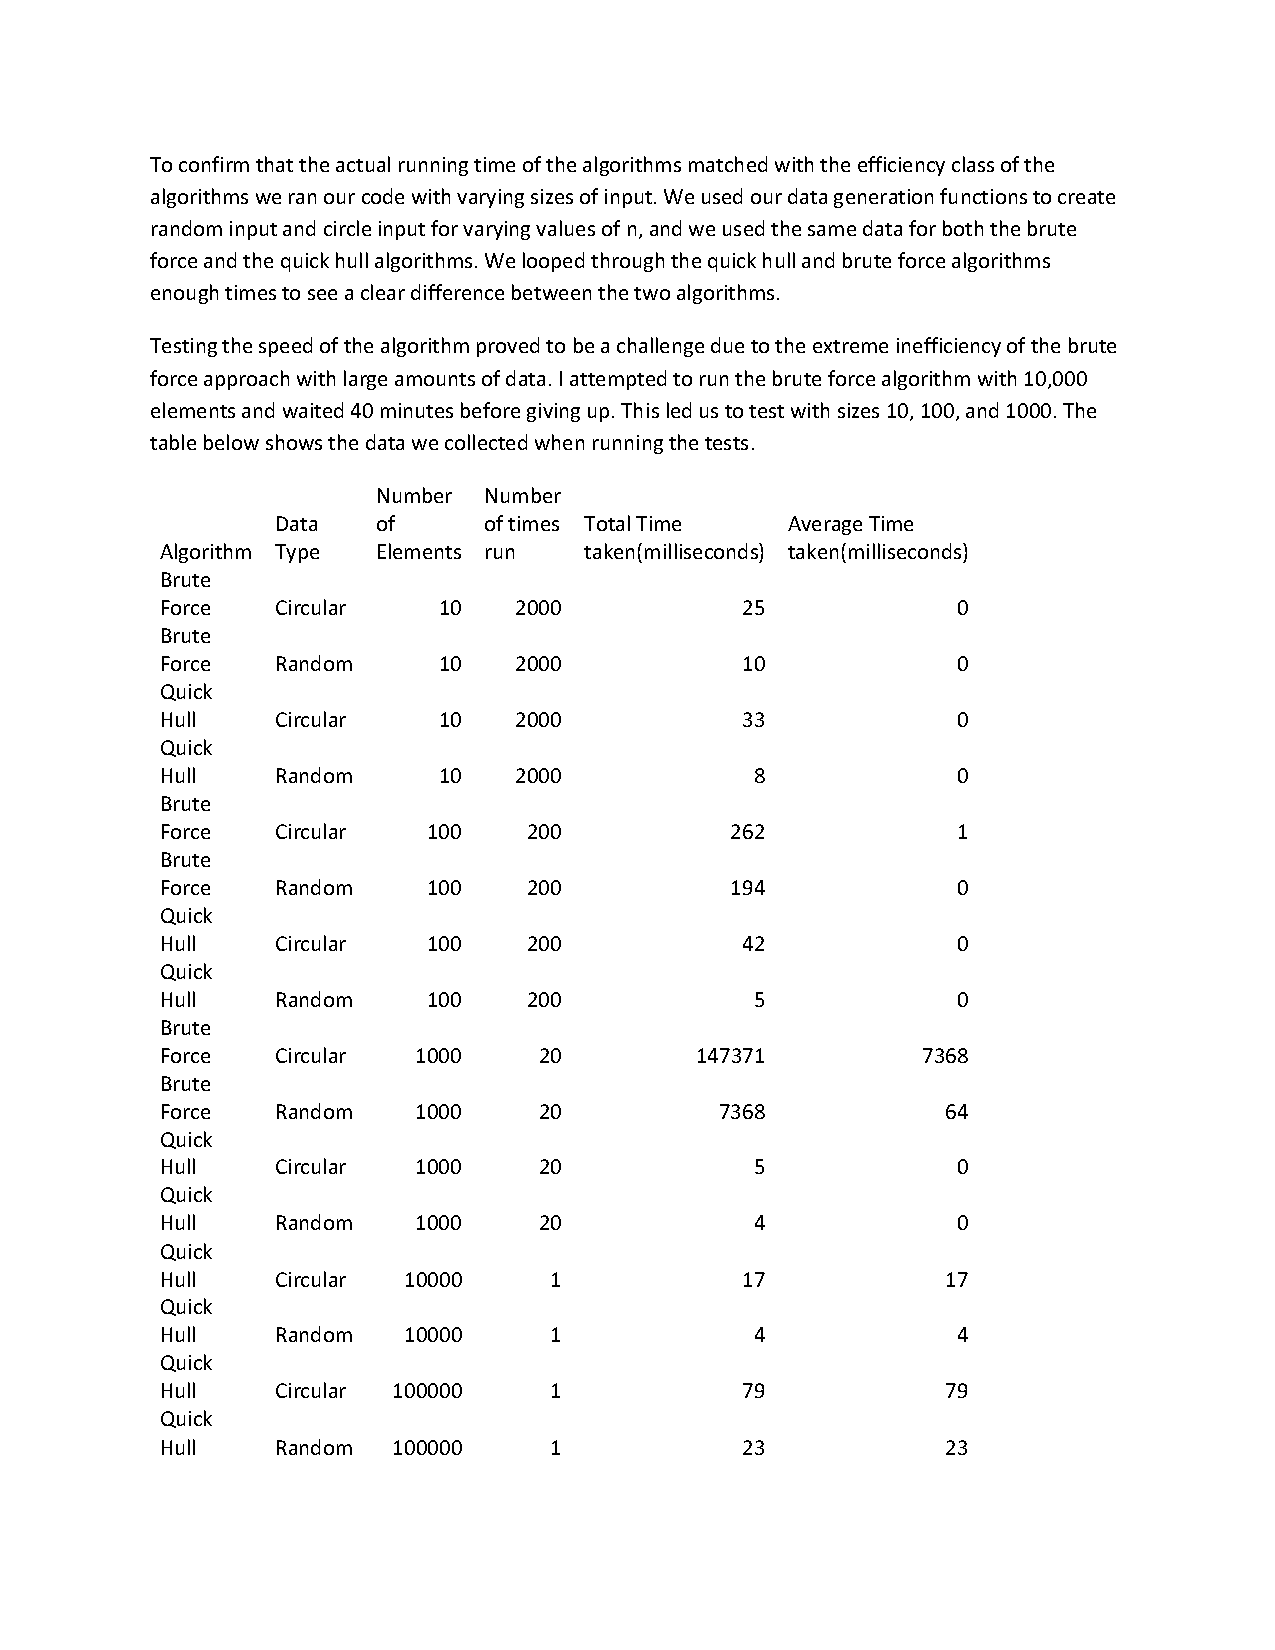
\includegraphics[width=15cm,height=16cm]{results.png}
  \end{center}
    \caption{Results}
    \label{fig:results}
  \end{figure} 
Looking at quick hull and comparing it with brute force with 10 elements shows very similar running
speeds, but as soon as 100 elements are tested the difference becomes apparent. The rate of growth
difference seems to be massive. With 100 elements of circular data brute force took 6 times longer to
run than quick hull, and at 1000 elements of circular data brute force took 29,474 times longer to run
than quick hull. While brute force took longer than 40 minutes to run before we quit the process on
10,000 elements quick hull took only 17 milliseconds.
\\\\
We expected the data generated in circular form to perform in n squared time for quick hull because it is
the worst case, and in n cubed time for brute force, so we assumed that the difference in running time
would be a factor of n. With 100 elements the factor was only 6, and with 1,000 elements the factor was
29,474, and these factors are very different than the factors of 100 and 1,000 that we expected. This
showed us that the performance of an algorithm with a specific efficiency class can vary drastically due
to implementation details, and although constant factors are ignored in efficiency classes they make a
big difference in practice.
\section{Conclusion}
We encountered a few issues where a lot of time was wasted due to poor planning and not exploring
our options. Our first attempt at correctness testing mimicked brute force too closely, and we realized
that comparing the data of our correctness testing and our brute force algorithm could miss certain
edge cases. Our first attempt at generating a circular set of points was also overly complicated, but
looking for better options ended with a simpler and more robust algorithm. We learned from this to
come up with multiple options before deciding on an implementation.
\\

Comparing the time taken to compute the convex hull using brute force and quick hull showed extreme
differences, and this solidified the importance of choosing an algorithm of the best known efficiency.
Most of the code that we have written so far through schooling has been tested on a small scale where
the difference in efficiency would not be noticeable, but the knowledge of how to analyze the
complexity of an algorithm and the importance of choosing a good algorithm will be invaluable.


  %----------------------------------------------------------------------------------------
  % BIBLIOGRAPHY
  %----------------------------------------------------------------------------------------

  \bibliographystyle{unsrt}

  \bibliography{sample}

  %----------------------------------------------------------------------------------------


\end{document}
